\documentclass{beamer}
\usepackage[polish]{babel}
\usepackage[utf8]{inputenc}
\usepackage[T1]{fontenc}
\usepackage{svg}
\usepackage{animate}
\usepackage{graphicx}
\usepackage{xcolor}
\usepackage{minted}
\usetheme{Madrid}
\usecolortheme{default}
%------------------------------------------------------------
%This block of code defines the information to appear in the
%Title page
\title[Praca dyplomowa magisterska] %optional
{Ocena jakości i wydajności generatora liczb losowych neoTRNG w układzie FPGA w zależności od konfiguracji oscylatorów pierścieniowych oraz zastosowanych ekstraktorów losowości}
\subtitle{}
\author[Szymon Gogulski] % (optional)
{Szymon~Krzysztof~Gogulski
\newline
\newline
Promotor: dr inż. Michał Melosik
\newline
\newline
Informatyka – Przetwarzanie Brzegowe
}
\institute[PP] % (optional)
{Politechnika Poznańska}
\date[Poznań 2026] % (optional)
{Praca dyplomowa magisterska
\newline
Poznań 2026}
\logo{
\includegraphics[height=0.6cm]{pp_logo.pdf}}
\begin{document}
\frame{\titlepage}
%---------------------------------------------------------
\begin{frame}
\frametitle{Agenda}
\tableofcontents
\end{frame}
%---------------------------------------------------------
\section{Cel pracy}
%---------------------------------------------------------
\begin{frame}
\frametitle{Cel pracy}

\LARGE

\begin{itemize}
    \item adaptacja oraz implementacja otwartoźródłowego generatora losowości neoTRNG,
    \item przeprowadzenie badań nad wpływem modyfikacji generatora na losowość.
\end{itemize}

\end{frame}
%---------------------------------------------------------
\section{Wprowadzenie}
%---------------------------------------------------------
\begin{frame}
\frametitle{Wprowadzone modyfikacje}

\LARGE

Aspekty generatora objęte modyfikacjami i badaniami:

\begin{itemize}
    \item liczba zastosowanych oscylatorów pierścieniowych (RO),
    \item zastosowanie korekcji źródła,
    \item metody przetwarzania końcowego,
    \item rozmieszczenie oscylatorów w strukturze FPGA.
\end{itemize}

\end{frame}
%---------------------------------------------------------
\begin{frame}
\frametitle{Kryteria oceny generatora}

\LARGE

\begin{itemize}
    \item zestaw testów statystycznych NIST SP 800-22,
    \item zestaw testów do oceny entropii minimalnej NIST SP 800-90B,
    \item program ENT.
\end{itemize}

\end{frame}
%---------------------------------------------------------
\begin{frame}
\frametitle{Model źródła}


    \begin{figure}[H]
      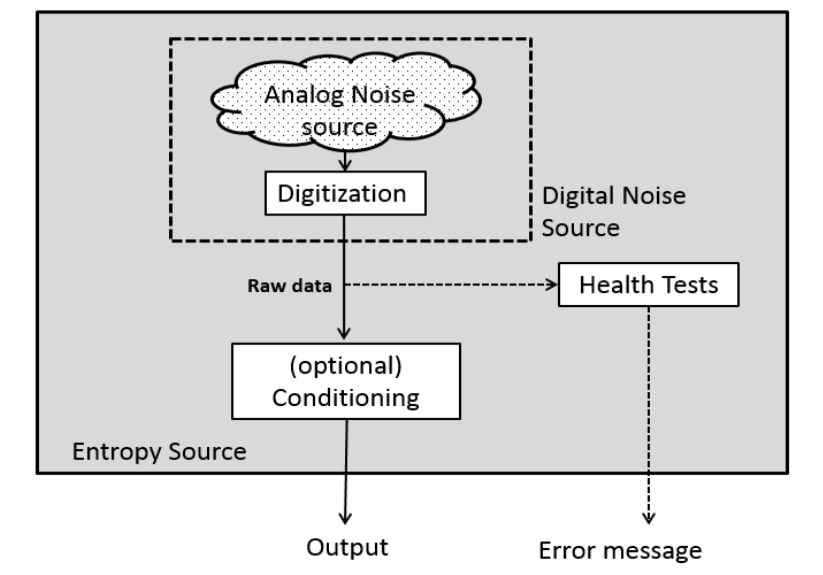
\includegraphics[width=0.75\textwidth]{figures/modle_zrodla.png}
      \caption{Model źródła entropii}
    \end{figure}

\stepcounter{footnote}\footnotetext[\value{footnote}]{\href{https://nvlpubs.nist.gov/nistpubs/SpecialPublications/NIST.SP.800-90B.pdf}{NIST SP 800-90B}}

\end{frame}
%---------------------------------------------------------
\begin{frame}
\frametitle{Oscylator pierścieniowy}

    \begin{figure}[H]
      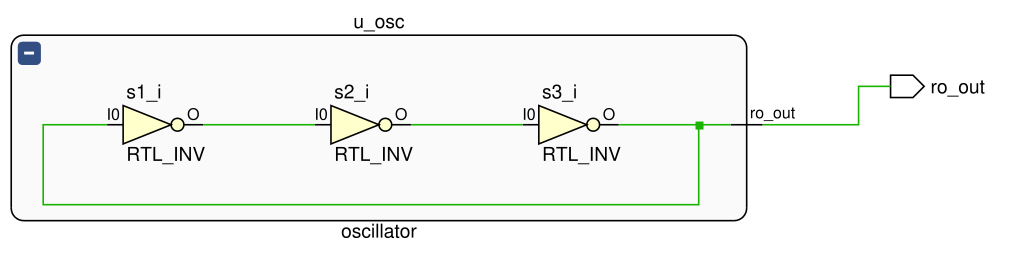
\includegraphics[width=\textwidth]{figures/oscylator.png}
      \caption{Prosty oscylator pierścieniowy}
    \end{figure}


\end{frame}
%---------------------------------------------------------
\begin{frame}
\frametitle{Architektura neoTRNG}

    \begin{figure}[H]
      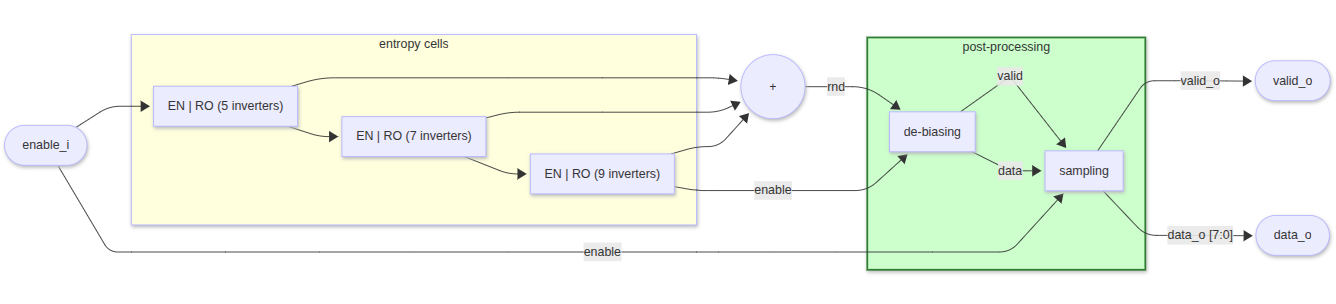
\includegraphics[width=\textwidth]{mermaid/png/2.png}
      \caption{Architektura modułu neoTRNG}
    \end{figure}

\end{frame}



%---------------------------------------------------------
\section{Wpływ liczby oscylatorów i liczby inwerterów}
%---------------------------------------------------------
\begin{frame}[fragile]
\frametitle{Wpływ liczby oscylatorów i liczby inwerterów}

\begin{minted}[linenos, breaklines, breakanywhere]{vhdl}
entity neoTRNG is
  generic (
    NUM_CELLS           : natural range 1 to 255;
    NUM_INV_START       : natural range 3 to 4095;
    NUM_RAW_BITS        : natural range 1 to 4096;
    SIM_MODE            : boolean;
    ENABLE_VON_NEUMANN  : boolean := true;
    ENABLE_CRC          : boolean := true
  );
end entity;
\end{minted}



\textbf{Czy skalowanie zasobów sprzętowych poprzez zwiększanie liczby RO oraz liczby inwerterów ma
kluczowe znaczenie dla jakości źródła entropii?}

\end{frame}
%---------------------------------------------------------
\begin{frame}
\frametitle{Wnioski}

\Large

\begin{itemize}
    \item zwiększenie liczby inwerterów przekłada się na poziom entropii,
    \item konfiguracje z większą liczbą RO/inwerterów nie zawsze gwarantują lepsze wyniki w testach NIST SP 800-22,
    \item zwiększenie entropii nie zwalnia z konieczności stosowania przetwarzania końcowego.
\end{itemize}

\end{frame}




%---------------------------------------------------------
\section{Efektywność przetwarzania końcowego von Neumanna oraz CRC}
%---------------------------------------------------------
\begin{frame}[fragile]
\frametitle{Efektywność przetwarzania końcowego von Neumanna oraz CRC}

\begin{minted}[linenos, breaklines, breakanywhere]{vhdl}
entity neoTRNG is
  generic (
    NUM_CELLS           : natural range 1 to 255;
    NUM_INV_START       : natural range 3 to 4095;
    NUM_RAW_BITS        : natural range 1 to 4096;
    SIM_MODE            : boolean;
    ENABLE_VON_NEUMANN  : boolean := true;
    ENABLE_CRC          : boolean := true
  );
end entity;
\end{minted}



    \textbf{Czy zastosowanie ekstraktora von Neumanna i wielomianu CRC w module neoTRNG ma znaczenie
dla jakości projektowanego generatora?}

\end{frame}
%---------------------------------------------------------
\begin{frame}
\frametitle{Wnioski}

\Large

\begin{itemize}
    \item wyłączenie zarówno korektora von Neumanna, jak i CRC, dyskwalifikuje generator w testach NIST SP 800-22,
    \item deaktywacja korektora von Neumanna przy aktywnym CRC zapewnia akceptowalną losowość.
\end{itemize}

\end{frame}












%---------------------------------------------------------
\section{Wpływ rozmieszczenia RO}
%---------------------------------------------------------
\begin{frame}
\frametitle{Wpływ rozmieszczenia RO}


\begin{figure}[H]
    \centering
    \begin{minipage}{0.48\textwidth}
        \centering
      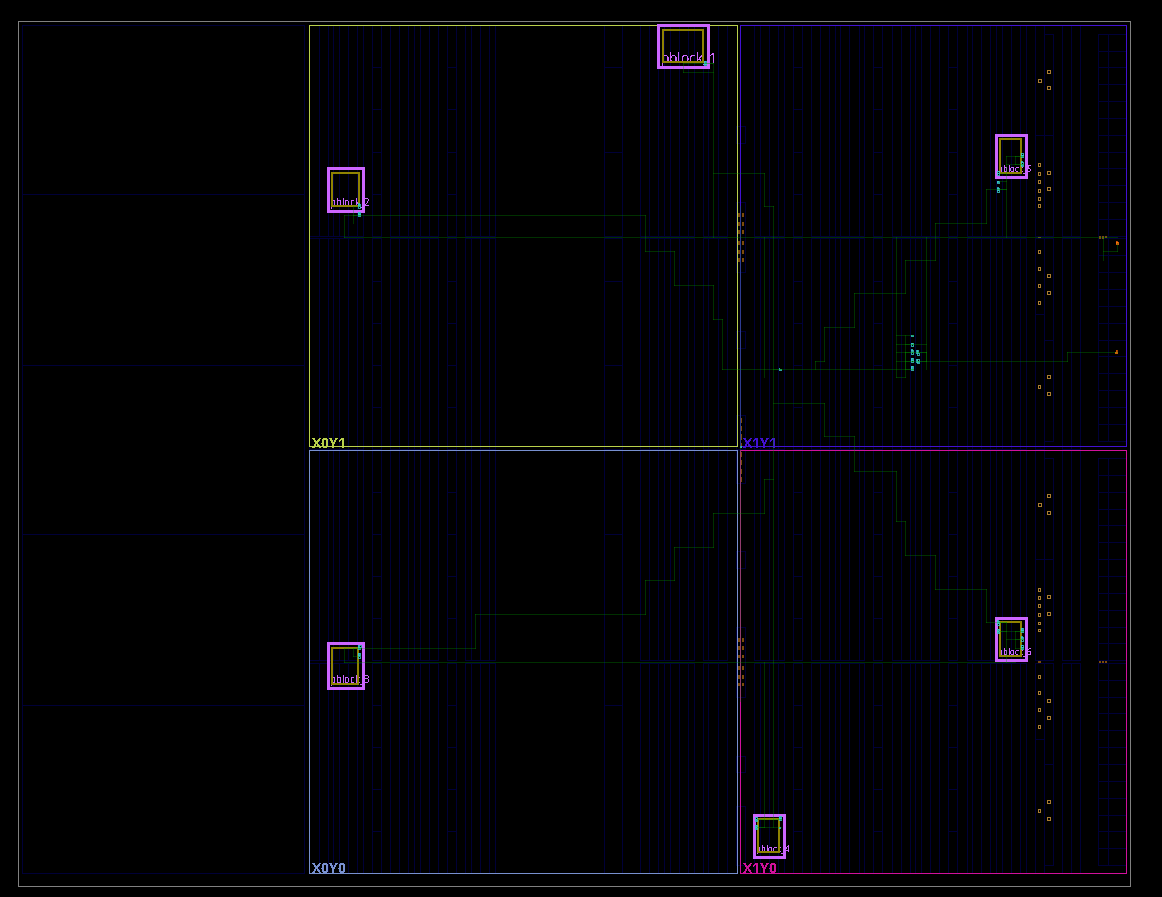
\includegraphics[width=\textwidth]{figures/ch4/6D2.png}
      \caption{Oscylatory rozproszone}
        \label{fig:ch4_2RO_distributed_screen}
    \end{minipage}
    \hfill % Adds horizontal space between the two figures
    \begin{minipage}{0.48\textwidth}
        \centering
      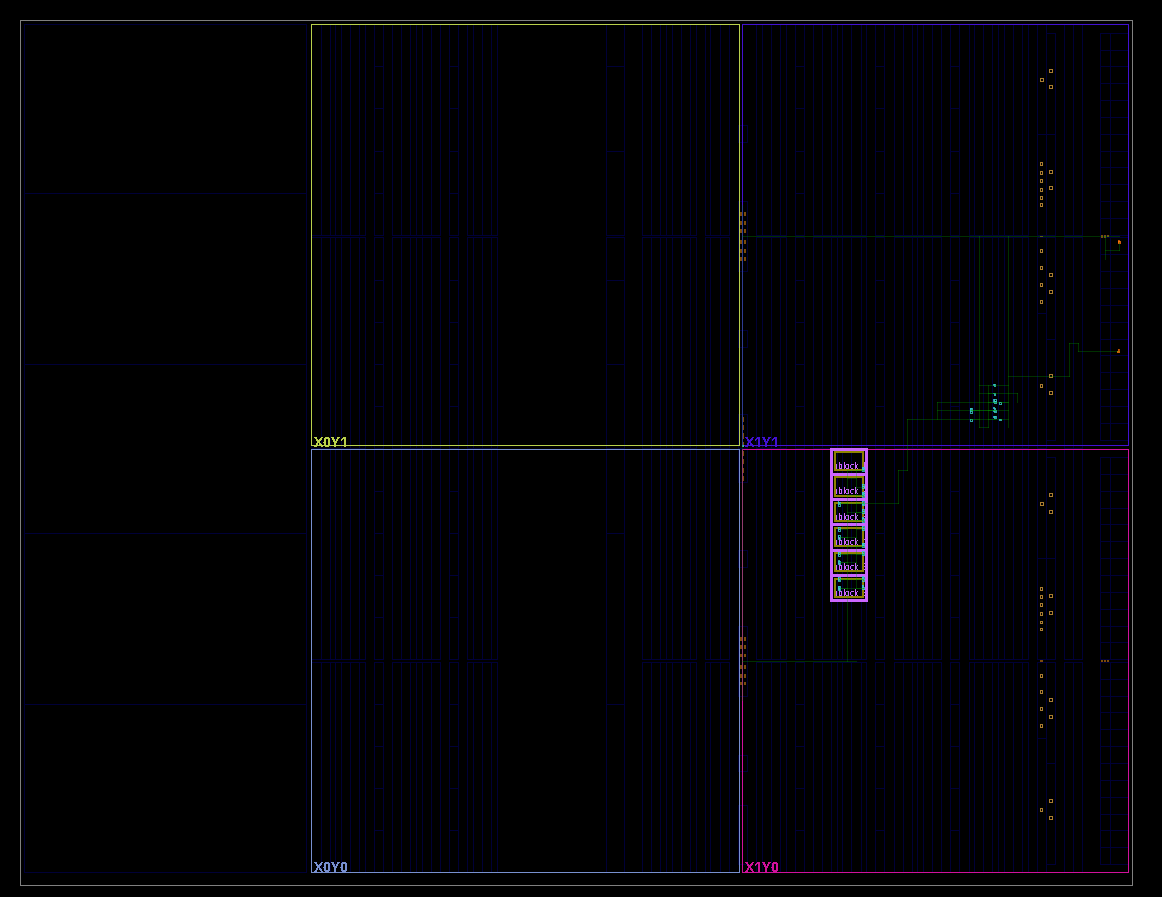
\includegraphics[width=\textwidth]{figures/ch4/6DL.png}
      \caption{Oscylatory zlokalizowane}
        \label{fig:ch4_2RO_localized_screen}
    \end{minipage}
\end{figure}

\textbf{Czy rozmieszczenie RO w strukturze FPGA ma istotne znaczenie dla jakości źródła?}

\end{frame}
%---------------------------------------------------------
\begin{frame}
\frametitle{Wnioski}

\Large

\begin{itemize}
    \item w ramach przeprowadzonych badań nie stwierdzono istotnego wpływu rozmieszczenia RO na losowość,
    \item sugerowane dalsze badania nad bardziej złożonym rozmieszczeniem w matrycy FPGA,
    \item przy rozmieszczeniu rozproszonym konfiguracja bez korektora von Neumanna (z aktywnym CRC) pozostaje efektywna.
\end{itemize}

\end{frame}










%---------------------------------------------------------
\section{Zastosowanie zaawansowanych metod przetwarzania końcowego}
%---------------------------------------------------------
\begin{frame}
\frametitle{Zastosowanie zaawansowanych metod przetwarzania końcowego}

\LARGE

  Zbadane metody przetwarzania końcowego:
  \begin{itemize}
    \item ekstraktor Toeplitza,
    \item szyfr strumieniowy AES-CTR.
  \end{itemize}

\vspace{1cm}
\normalsize
\textbf{Czy zaawansowane metody przetwarzania końcowego mają przewagę nad metodami bazowymi?}

\end{frame}
%---------------------------------------------------------
\begin{frame}
\frametitle{Zaawansowane metody przetwarzania końcowego – wnioski}

\Large

\begin{itemize}
    \item AES-CTR i Toeplitz przeszły pomyślnie testy statystyczne,
    \item AES-CTR zwiększa wydajność kosztem zasobów bez utraty jakości,
    \item ekstraktor Toeplitza stanowi optymalny kompromis wydajnościowy,
    \item ze względu na silne algorytmy kryptograficzne zaleca się implementację z użyciem AES-CTR.
\end{itemize}

\end{frame}












%---------------------------------------------------------
\section{Podsumowanie}
%---------------------------------------------------------
\begin{frame}
\frametitle{Podsumowanie}

\Large

\begin{itemize}
    \item kluczem do optymalnego TRNG jest balans między wykorzystaniem zasobów, rozmieszczeniem RO, doborem ekstraktora i przeprowadzeniem testów,
    \item błędna adaptacja (pominięcie ekstraktorów) prowadzi do niskiej jakości losowości,
    \item implementacja parzystej liczby inwerterów z korektorem von Neumanna może zatrzymać proces kryptograficzny.
\end{itemize}

\end{frame}
%---------------------------------------------------------
\begin{frame}
\frametitle{}
\centering{\Huge{\textbf{Dziękuję za uwagę}}}
\end{frame}
%---------------------------------------------------------
\end{document}